\documentclass[aspectratio=169,xcolor=dvipsnames]{beamer}
\usepackage[utf8]{inputenc}  % Required for umlauts
\usepackage[english]{babel}  % Language
%\usepackage[sfdefault]{roboto}  % Enable sans serif font roboto
%\usepackage{libertine}  % Enable this on Windows to allow for microtype
\usepackage[T1]{fontenc}  % Required for output of umlauts in PDF

\usepackage{mathtools,bbold}  % Required for formulas
\usepackage{siunitx}  % Give numbers units (with proper spacing)

\usepackage{caption}  % Customize caption aesthetics
\usepackage{tcolorbox}  % Fancy colored boxes
\usepackage{color}
\usepackage{xcolor}  % Highlighting
\usepackage{soul}

\usepackage{booktabs}  % Using pandas' LaTeX output
\usepackage{multirow}  % Enable fancy table structure
\usepackage{listings}  % Insert programming code
\usepackage{lstautogobble}  % Cleaner indentation in TeX file of code blocks within LaTeX blocks

\usepackage{graphicx}  % Required to insert images
\usepackage{subcaption}  % Enable sub-figure
\usepackage[space]{grffile}  % Insert images baring a filename which contains spaces
\usepackage{float}  % Allow to forcefully set the location of an object
% Include external standalone files such as Tikz graphics; requires `-shell-escape`
\usepackage{standalone}
\usepackage{tikz}  % Fancy drawing environment
\usepackage{pgfplots}  % Functions in Tikz
\usepackage[]{algorithm2e}  % Format fancy algorithms

\usepackage[tracking=true]{microtype} % Required to change character spacing

\usepackage[backend=biber,autocite=footnote,style=authoryear-icomp,sorting=none,doi=false,isbn=false,url=false,eprint=false]{biblatex}
\usepackage{csquotes}  % Ensure proper quotation of texts with babel and polyglossia with biblatex
\usepackage{hyperref}  % Insert clickable references

\usepackage{datetime}  % Flexible date specification

\usepackage{geometry}
\usepackage{scrextend}  % Allow arbitrary indentation

\usepackage{appendixnumberbeamer}  % Fancy page numbering excluding the appendix

% Compile notes into a separate file readable by pdfpc using a custom package which overwrite the `note` macro
\usepackage{pdfpcnotes}
% NOTE: Adding "noframenumbering" as argument to the first slide confuses `pdfpc`; see https://github.com/pdfpc/pdfpc/issues/367

\usetikzlibrary{patterns}
\usetikzlibrary{arrows}
\usetikzlibrary{matrix}
\usetikzlibrary{hobby}
\usetikzlibrary{shapes.misc}
\usetikzlibrary{shapes.callouts}
\pgfmathdeclarefunction{gauss}{2}{%
	\pgfmathparse{1/(#2*sqrt(2*pi))*exp(-((x-#1)^2)/(2*#2^2))}%
}

\addbibresource{literature.bib}
\renewcommand{\footnotesize}{\tiny}
%\renewcommand*{\bibfont}{\scriptsize}

\newcommand{\leadingzero}[1]{\ifnum#1<10 0\the#1\else\the#1\fi}
\newcommand{\todayddmmyyyy}{\leadingzero{\day}.\leadingzero{\month}.\the\year}
\newcommand{\mathcolorbox}[2]{\colorbox{#1}{$\displaystyle #2$}}

\DeclareMathOperator*{\argmin}{arg\,min}

\makeatletter
% Fix subfig in beamer style presentation
\let\@@magyar@captionfix\relax

% Insert [short title] for \section in ToC
\patchcmd{\beamer@section}{{#2}{\the\c@page}}{{#1}{\the\c@page}}{}{}
% Insert [short title] for \section in Navigation
\patchcmd{\beamer@section}{{\the\c@section}{\secname}}{{\the\c@section}{#1}}{}{}
% Insert [short title] for \subsection in ToC
\patchcmd{\beamer@subsection}{{#2}{\the\c@page}}{{#1}{\the\c@page}}{}{}
% Insert [short title] for \subsection in Navigation
\patchcmd{\beamer@subsection}{{\the\c@subsection}{#2}}{{\the\c@subsection}{#1}}{}{}
\makeatother

\definecolor{dodgerblue}{rgb}{0.06, 0.44, 0.8}
\setbeamercolor{tableofcontents}{fg=dodgerblue}
\setbeamercolor{section in toc}{fg=black}
\setbeamercolor{subsection in toc}{fg=black}
\setbeamercolor{block title}{fg=black}
\setbeamercolor{qed symbol}{fg=black}
\setbeamercolor{enumerate item}{fg=black}
\setbeamercolor{itemize item}{fg=black}
\setbeamercolor{itemize subitem}{fg=black}
\setbeamercolor{title}{fg=dodgerblue}
\setbeamerfont{title}{size=\LARGE}
\setbeamertemplate{title page}{%
	\vbox{}
	\begin{centering}
		\begin{beamercolorbox}[sep=8pt,center]{title}
			\usebeamerfont{title}\inserttitle\par%
			\ifx\insertsubtitle\@empty%
			\else%
				\vspace{0.25em}
				{\usebeamerfont{subtitle}\usebeamercolor[fg]{subtitle}\insertsubtitle\par}%
			\fi%
		\end{beamercolorbox}%
		\vspace{1em}\par
		\begin{beamercolorbox}[sep=8pt,center]{author}
			\usebeamerfont{author}\insertauthor%
		\end{beamercolorbox}
		\begin{beamercolorbox}[sep=8pt,center]{institute}
			\usebeamerfont{institute}\insertinstitute%
		\end{beamercolorbox}
		\begin{beamercolorbox}[sep=8pt,center]{date}
			\usebeamerfont{date}\insertdate%
		\end{beamercolorbox}%\vskip0.5em
	\end{centering}
}
\setbeamercolor{frametitle}{fg=dodgerblue}
\setbeamerfont{frametitle}{size=\LARGE}
\setbeamerfont{framesubtitle}{size=\small}
\setbeamertemplate{frametitle}{%
	\nointerlineskip%
	\hspace*{0.45em}
	% Other decent options are: `center`
	\begin{beamercolorbox}[ht=4em,sep=1em,wd=\paperwidth]{frametitle}
		\usebeamerfont{framesubtitle}
		\hspace{-0.3em}\strut\insertframetitle\strut%
		\\
		\usebeamerfont{frametitle}
		\strut\insertframesubtitle\strut%
	\end{beamercolorbox}
}
\setbeamercolor{footline}{fg=gray}
\setbeamercolor{date in head/foot}{fg=gray}
\setbeamercolor{author in head/foot}{fg=gray}
\setbeamercolor{section in head/foot}{fg=gray}
\setbeamerfont{footline}{size=\tiny}
\setbeamertemplate{footline}[text line]{%
	\leavevmode%
	\hspace*{-3.2em}
	\hbox{%
		\begin{beamercolorbox}[wd=.33\paperwidth,ht=1em,dp=0.5em,left]{date in head/foot}%
			\hspace{1.5em}
			\usebeamerfont{date in head/foot}\insertshortdate
		\end{beamercolorbox}%
		\begin{beamercolorbox}[wd=.33\paperwidth,ht=1em,dp=0.5em,center]{author in head/foot}%
			\usebeamerfont{author in head/foot}\insertshortauthor
		\end{beamercolorbox}%
		\begin{beamercolorbox}[wd=.33\paperwidth,ht=1em,dp=0.5em,right]{section in head/foot}%
			\usebeamerfont{date in head/foot}
			\insertframenumber{} %/ \inserttotalframenumber\hspace*{1em}  % NOTE, excessive for a 12 min. talk
			\hspace{1.5em}
		\end{beamercolorbox}
	}
}
\setbeamertemplate{navigation symbols}{}
\setbeamertemplate{itemize item}{$\bullet$}
\setbeamertemplate{itemize subitem}{$\circ$}
\captionsetup{font=scriptsize,labelfont={bf,scriptsize}}

% Customize code blocks
\definecolor{dodgerblue}{rgb}{0.06, 0.44, 0.8}
\definecolor{dodgerred}{rgb}{0.93, 0.24, 0.26}
\lstset{basicstyle=\ttfamily,
	breaklines=true,
	showstringspaces=false,
	commentstyle=\color{dodgerred},
	keywordstyle=\color{dodgerblue},
	frame=none,
	frameround=ffff,
	autogobble=true
}
\lstset{language=Python,
	basicstyle=\ttfamily\scriptsize,
	rulecolor=\color{black},
	tabsize=2,
}

\title{NIFTy: The Why and How of Building AD from Scratch}
\subtitle{}
\author[Gordian Edenhofer]{%
	{\href{mailto:gordian.edenhofer@gmail.com}{Gordian Edenhofer}}\inst{1,2,3}
}
\institute[LMU]{%
	\inst{1}Max Planck Institute for Astrophysics, Garching \\
	\inst{2}Faculty of Physics, LMU, Munich \\
	\inst{3}Center for Astrophysics $\vert$ Harvard \& Smithsonian, Boston \\
}
\date[EnzymeCon]{Enzyme Conference 2023, \formatdate{23}{02}{2023}}
\subject{}

\begin{document}

% NOTES
% * Introduce myself!!!
% * Do NOT talk about TOC for a 12 min. talk

\pagenumbering{arabic}

\begin{frame}[plain]
	\titlepage%
	\note{%
		* From astrometric and photometric data to 3D dust
	}
\end{frame}

% Submitted Abstract
%
% Automatic Differentiation (AD) is the backbone of applied second order
% minimization schemes and used extensively for solving statistical inference
% problems. Both often require forward and reverse mode differentiation for
% efficiency. However, early AD frameworks did not support both. In 2013 this
% sparked the development of NIFTy, a Bayesian inference library with a
% (specialized) second order minimization scheme and a custom-built AD engine on
% top of NumPy. In this talk we introduce how NIFTy realizes AD via
% linearization- and transposition-rules. Furthermore, we discuss how using AD
% for second order minimization affects the choice of rematerialization
% strategies. Attendees will learn core concepts for building their own simple
% AD framework and why linearizations and transpositions are highly desirable
% for efficient second order minimization.

\section{AD in Astrophysical Imaging}  % Background
\frame[plain,noframenumbering]{\vfill\centering\tableofcontents[sectionstyle=show/shaded,subsectionstyle=show/hide]\vfill}

\subsection{What}  % Introduction, Background
{
\setbeamercolor{background canvas}{bg=black}
\begin{frame}[plain,noframenumbering]
	\begin{tikzpicture}[overlay, remember picture, every text node part/.style={align=center}]
		\node[anchor=north west,xshift=-0.15cm,yshift=-0.25cm] at (current page.north west)
		{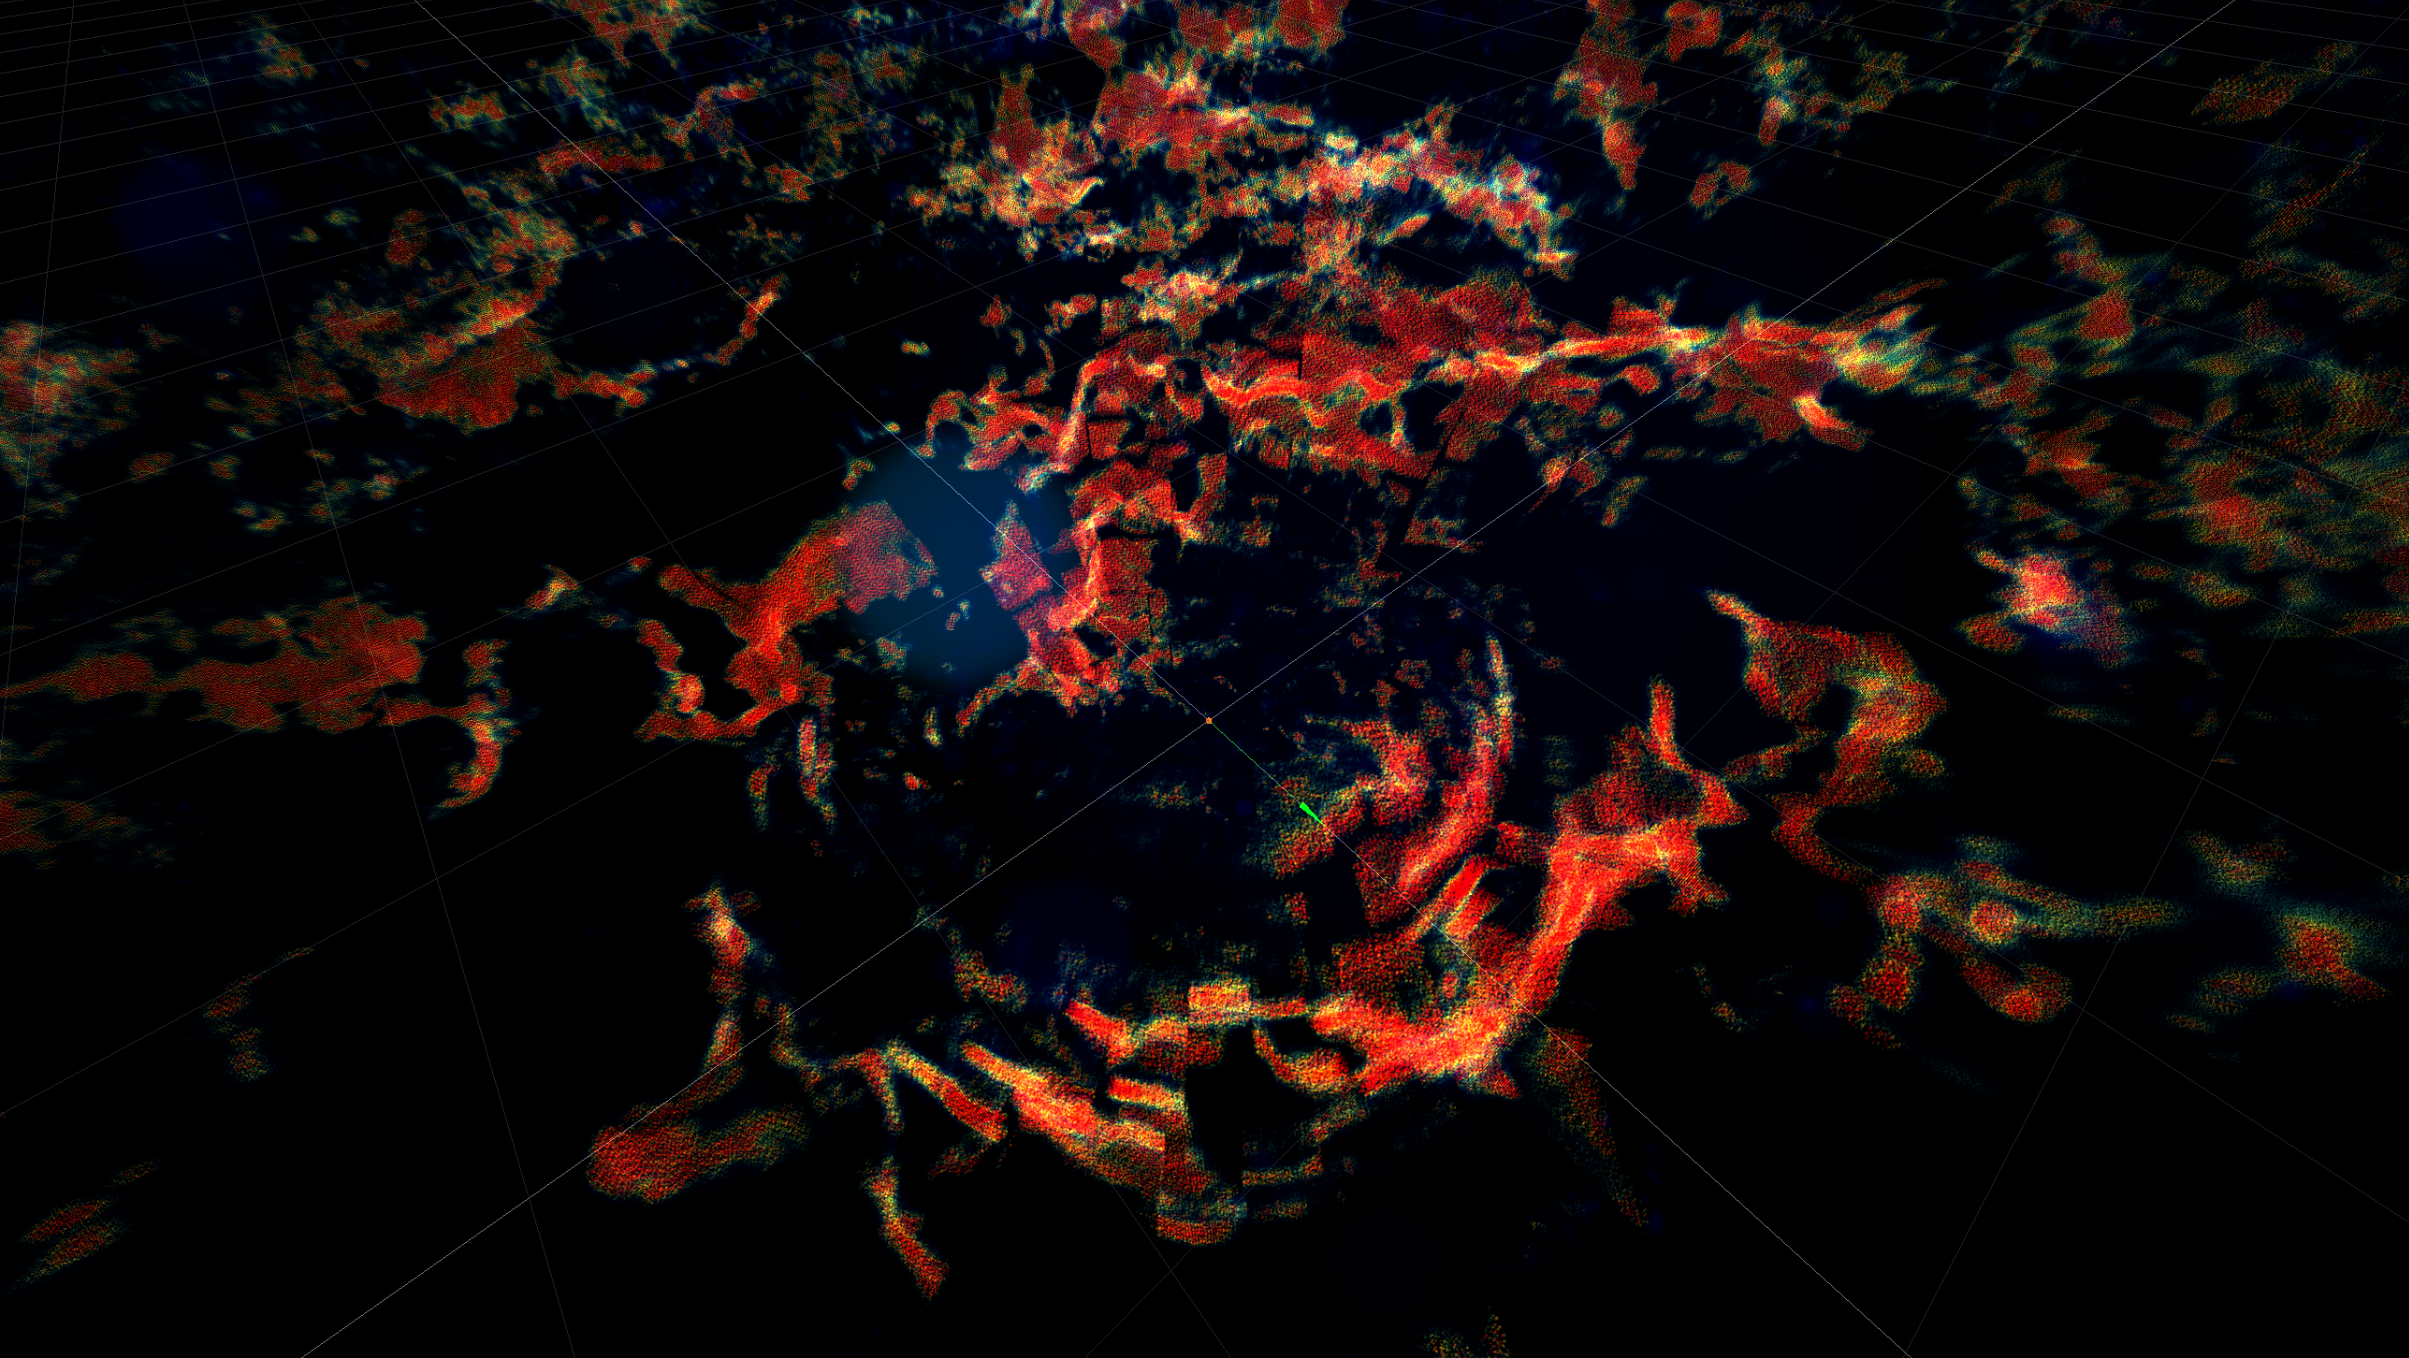
\includegraphics[width=1.145\textwidth,keepaspectratio]{{res/galactic_dust_off_axis_perspective}}};
	\end{tikzpicture}

	\note{* What I really want to do is 3D dust mapping}
	\note{* Meaning: statistical inference on lots of data with complicated model}
	\note{* 10M data points that can not simply be batched like in ML but need to be processed jointly}
	\note{* I want to do statistical inference}
	\note{* Our approach to do so is by solving big optimization problem}
	\note{* Optimizations get faster if one uses derivates}
\end{frame}
}

\begin{frame}
	\frametitle{\insertsection}
	\framesubtitle{\insertsubsection}

	\begin{itemize}
		\item Statistical inference on $10+$M dofs $\rightarrow$ optimizing cost function
		\item Cost function of data $d$ and parameters $x$
		\begin{align*}
			H(x) &= \ell'(d, x) + x^2
			\\ &= \ell(f(x)) + x^2
		\end{align*}
		\item From theory: Hessian $H''(x, y) \approx J_f^\dagger \hat{L'} J_f + 1$ {\footnotesize\color{gray}with $J_f$ the Jacobian of $f$ and some simple matrix $\hat{L'}$}
		% \pause
		\item[$\rightarrow$] $2^\text{nd}$ order minimization
	\end{itemize}

	\note{* split of cost function is important}
	\note{* having to use full data + easily accessible Hessian approx. screams for second order AD}
\end{frame}

\subsection{Problems}  % Problem, Goal
\begin{frame}
	\frametitle{\insertsection}
	\framesubtitle{\insertsubsection}

	\begin{itemize}
		\item Many ($\approx10^4$) calls to $H''(x, y) \approx J_f^\dagger \hat{L'} J_f + 1$, few ($\approx10^3$) to $\nabla_x H(x)$
		\item Special in that applies linear operator $J$ but few non-linearities
		\item Few AD toolkits cater to need for efficient $J$
		% \item[$\rightarrow$] More than just gradients
	\end{itemize}

	\begin{center}
		Numerical Information Field Theory = DIY AD + (bunch of statistics)
	\end{center}

	\note{* specialized 2nd order minimization}
	\note{* NIFTy custom AD for fast Hessian application}
	\note{* rest of the talk will focus on how we do this and what makes it efficient for our kind of problems}
	% \footcitetext{Selig2013,Steiniger2019}
\end{frame}

\section{Linearizations on top of NumPy}  % Methodology
\frame[plain,noframenumbering]{\vfill\centering\tableofcontents[sectionstyle=show/shaded,subsectionstyle=show/hide]\vfill}

\subsection{Example}
\begin{frame}
	\frametitle{\insertsection}
	\framesubtitle{\insertsubsection}

	% TODO: merge sum and weighting into weighted sum? and include correlated_field

	\begin{equation*}  % TODO: built up successively
		f(x) =
		\sum_0^m
		\circ
		\ \text{weight}
		\circ
		\exp
		\circ
		\begin{bmatrix}
			x_{00} & \dots & x_{0m} \\
			\vdots & \ddots & \\
			x_{n0} & \dots & x_{nm}
		\end{bmatrix}
	\end{equation*}

	\vspace{1em}
	\begin{center}
		Constraints: skip non-linearities in $J_f$ and always compute weight on the fly
	\end{center}

	\note{* physics inspired model}
	\note{* constraints are essential}
	\note{* even current state-of-the-art AD models fail to fulfill them}
	\note{* complain about JAX}
\end{frame}

\subsection{Idea}
\begin{frame}
	\frametitle{\insertsection}
	\framesubtitle{\insertsubsection}

	Built implicit linear operator for Jacobian of f $J_f$ and its transpose $J_f^\dagger$
	\vspace{1em}
	\\ Constraints: skip non-linearities in $f$ and always compute weight on the fly

	\vspace{3em}
	\begin{columns}[T]
		\begin{column}{0.48\textwidth}
			\centering Forward mode (naive $J_f$)
			\begin{itemize}
				\item No memory overhead
				\item Re-evaluating non-linearities
			\end{itemize}
		\end{column}
		\begin{column}{0.48\textwidth}
			\centering Reverse mode (naive $J_f^\dagger$)
			\begin{itemize}
				\item Memory overhead
				\item No re-evaluating of non-linearities
			\end{itemize}
		\end{column}
	\end{columns}

	\note{* we want transpose of reverse mode}
	\note{* but configurable reverse mode to compute parts on the fly}
\end{frame}

\begin{frame}
	\frametitle{\insertsection}
	\framesubtitle{\insertsubsection}

	NIFTy
	\begin{enumerate}
		\item Associate every non-linearity with a corresponding linearization $J$ and $J^\dagger$
		\item Use the chain-rule to built up an AD toolkit
	\end{enumerate}

	\note{* Transposed of backwards pass for efficient forward AD}
	\note{* non-linearities are made much cheaper here; imagine e.g. and exp in the forward model}
\end{frame}

\begin{frame}
	\frametitle{\insertsection}
	\framesubtitle{\insertsubsection}

	\begin{equation*}
		f(x) =
		\sum_0^m
		\circ
		\ \text{weight}
		\circ
		\exp
		\circ
		\begin{bmatrix}
			x_{00} & \dots & x_{0m} \\
			\vdots & \ddots & \\
			x_{n0} & \dots & x_{nm}
		\end{bmatrix}
	\end{equation*}

	$\sum_0^m$: $\sum_0^m$, outer-product
	\\ weight: weight, adjoint weigthing
	\\ $\exp$: multiplication with $\exp(x^{(0)})$, multiplication with $\exp(x^{(0)})$

	\vspace{2em}

	$J_f = TODO$
	\\ $J_f^\dagger = TODO$

	\note{* this has been rediscovered over and over; there is a dedicated JAX paper on this...}
\end{frame}

\subsection{Linearizations}
\begin{frame}[fragile]
	\frametitle{\insertsection}
	\framesubtitle{\insertsubsection}

	\begin{lstlisting}[language=python,escapechar=!]
		class Linearization():
			def __init__(self, primals, fwd=lambda x: x, bwd=lambda y: y):
				self.p = primals
				self._fwd, self,_bwd = fwd, bwd

			def __call__(self, primals):
				return self._fwd(primals)

			@property
			def T(self):
				return self.__class__(None, self._bwd, self._fwd)
	\end{lstlisting}

	\note{* linearization needs to know position as to amend it}
	\note{* linearization needs to forward pass = J_f}
	\note{* linearization needs to backward pass = J_f^+}
\end{frame}

\begin{frame}[fragile]
	\frametitle{\insertsection}
	\framesubtitle{\insertsubsection}

	\begin{lstlisting}[language=python,escapechar=!]
		def exp(self, pl):
			if isinstance(pl, Linearization):
				y = np.exp(pl.p)
				fwd = lambda y: x_new * pl(y)
				bwd = lambda y_T: pl.T(y_T) * x_new
				return Linearization(y, fwd, bwd)
			return np.exp(pl)
	\end{lstlisting}

	\begin{lstlisting}[language=python,escapechar=!]
		x0 = np.arange(3, 3)
		y = exp(x0)
		j = exp(Linearization(x0))

		j = TODO
	\end{lstlisting}

	\note{* Note how the linearization and its adjoin is successively amended}
	\note{* Amending relies on closures}
\end{frame}

\begin{frame}
	\frametitle{\insertsection}
	\framesubtitle{\insertsubsection}

	\begin{enumerate}
		\item[$\checkmark$] Associate every non-linearity with a corresponding linearization $J$ and $J^\dagger$
		\item[$\checkmark$] Use the chain-rule to built up an AD toolkit
	\end{enumerate}

	\note{* linearization differ from JVP/VJP in that they do not evaluate the original function}
\end{frame}

\begin{frame}[fragile]
	\frametitle{\insertsection}
	\framesubtitle{\insertsubsection}

	\begin{equation*}
		f(x) =
		\sum_0^m
		\circ
		\ \text{weight}
		\circ
		\exp
		\circ
		\begin{bmatrix}
			x_{00} & \dots & x_{0m} \\
			\vdots & \ddots & \\
			x_{n0} & \dots & x_{nm}
		\end{bmatrix}
	\end{equation*}

	$\sum_0^m$: $\sum_0^m$, outer-product
	\\ weight: weight, adjoint weigthing
	\\ $\exp$: multiplication with $\exp(x^{(0)})$, multiplication with $\exp(x^{(0)})$

	\vspace{2em}

	$J_f = TODO$
	\\ $J_f^\dagger = TODO$

	\note{* get back to original demo of chained cost function}
	\note{* get linearizations by putting linearization into model and successively amending it}
\end{frame}

\subsection{Linearizations for minimization objective}
\begin{frame}[fragile]
	\frametitle{\insertsection}
	\framesubtitle{\insertsubsection}

	\begin{lstlisting}[language=python,escapechar=!]
		def exp(self, pl):
			...

		def weight(self, pl):
			...

		def sum(self, pl):
			...
	\end{lstlisting}

	\begin{lstlisting}[language=python,escapechar=!]
		f = lambda x: sum(weight(exp(x)))

		x0 = np.ones(3, 4)
		y, jac = f(Linearization(x0, lambda x: x, lambda x: x))
		jac(x0)
		jac.T(y)
	\end{lstlisting}

	\note{* congrats, you now understand the DIY AD in NIFTy}
\end{frame}

\subsection{Checkpointing}
\begin{frame}
	\frametitle{\insertsection}
	\framesubtitle{\insertsubsection}

	Checkpointing a.k.a. rematerialization strategy = storing versus recomputing values required for AD

	\begin{itemize}
		\item Crucial as \#parameter and constants in astrophysical models can be huge
		\item $J_f$ and $J_f^\dagger$ can almost always share constants
		\item Computation versus memory tradeoff impossible in general $\rightarrow$ needs user input
	\end{itemize}

	\note{* DIY in NIFTy}
	\note{* Memory versus computation tradeoff }
	\note{* looking at you JAX for excessive memory allocation for transpositions}
\end{frame}

\begin{frame}[fragile]
	\frametitle{\insertsection}
	\framesubtitle{\insertsubsection}

	\begin{lstlisting}[language=python,escapechar=!]
		def weight(self, pl):
			if isinstance(pl, Linearization):
				def fwd(x): return weight(pl(x))
				def bwd(x): return weight(pl.T(x))
				return Linearization(pl(x), fwd, bwd)
			# Super memory-intensive computation that should be
			# rematerialization at all costs
			weights = np.linspace(1, 10, pl.size).reshape(pl.shape)
			return weights * pl
	\end{lstlisting}
\end{frame}

\section{Numerical Information Field Theory}  % Result
\frame[plain,noframenumbering]{\vfill\centering\tableofcontents[sectionstyle=show/shaded,subsectionstyle=show/hide]\vfill}

% \subsection{Linearizations in NIFTy}
% \begin{frame}
% 	\frametitle{\insertsection}
% 	\framesubtitle{\insertsubsection}

% 	NIFTy is designed for large statistical models with 10+M dofs
% 	\vspace{1em}
% 	Computational cost dominated Hessian calls
% 	\vspace{1em}
% 	Hessian calls dominated by few inherently expensive operations (often \texttt{FFT})
% 	\vspace{1em}
% 	Fast if individal computations are expensive and done efficiently outside of python
% \end{frame}


\subsection{NIFTy AD}
\begin{frame}[fragile]
	\frametitle{\insertsection}
	\framesubtitle{\insertsubsection}

	\begin{lstlisting}[language=python,escapechar=!]
		correlated_field = ...
		model = ift.ContractionOperator(correlated_field.target) \
		@ weight \
		@ ift.exp \
		@ correlated_field

		j = model(ift.Linearization.make_var(x))
	\end{lstlisting}

	\note{* NIFTy is made for astrophysical inference}
	\note{* NIFTy implements custom posterior approximation techniques}
	\note{* NIFTy implements cool modeling tools for representing smoothness, e.g. for dust clouds}
\end{frame}

\subsection{Advantages of NIFTy-like Linearizations}
\begin{frame}
	\frametitle{\insertsection}
	\framesubtitle{\insertsubsection}

	\begin{itemize}
		\item Convenience of python
		\item Fast if individual computations are fast
		\item Easy to amend and include custom code
	\end{itemize}

	\note{* make bottle necks go brrr with C++}
	\note{* this is how we infer models with 10+M parameters}
\end{frame}

\end{document}
